\documentclass{article}
    % General document formatting
    \usepackage[margin=0.7in]{geometry}
    \usepackage[parfill]{parskip}
    \usepackage[utf8]{inputenc}
    \usepackage{graphicx}
    \graphicspath{ {../assets/} }
    
    % Related to math
    \usepackage{amsmath,amssymb,amsfonts,amsthm}

\begin{document}

\section*{Rotation}
\centerline{a is the anchor in the anchor point in the body's object space}
\centerline{theta is the body's rotation matrix}

\begin{gather}
u = v + \theta \cdot a \\
\theta = 
\begin{bmatrix}
    cos(t) & -sin(t) \\ 
    sin(t) & cos(t)
\end{bmatrix} \\
\omega = \frac{d\theta}{dt} =
\begin{bmatrix}
    -sin(t) & -cos(t) \\ 
    cos(t) & -sin(t)
\end{bmatrix} \\
a \cdot \theta = 
\begin{bmatrix}
a _x \cdot cos(t) + a _y \cdot -sin(t) \\
a _x \cdot sin(t) + a _y \cdot cos(t) \\
\end{bmatrix} \\
a \cdot \omega = 
\begin{bmatrix}
a _x \cdot -sin(t) + a _y \cdot -cos(t) \\
a _x \cdot cos(t) + a _y \cdot -sin(t) \\
\end{bmatrix} \\
\end{gather}
A vector times the time derivative of a rotation matrix is just the vector times the rotation matrix rotated by \(\frac{\tau}{4}\). This makes sense, because for a point to rotate around a center it has to be perpendicular to the center which means it's velocity is it's position rotated rotated by \(\frac{\tau}{4}\). Doing this is essentially the same treating the 2D plane as part of 3D space and taking the cross product of the $ \begin{bmatrix} 0 & 0 & \omega \end{bmatrix} $ where omega is the angular velocity with the point on the circle. \\
A generalization of this to n dimensional space is the geometric algebra left contraction operator. Which in a way removes a vector from the angular velocity bivector, which gives another vector. \\
This only describes the rotation at the angular speed of 1. If the angular speed is $a$ then this means the functions in the $\theta$ matrix take $ a \cdot t $ as the argument so by the chain rule the derivative gets scaled by $a$. When a vector spins $a$ times faster then the velocity vector is $a$ times longer.

$\boldsymbol\theta$ is the rotation matrix that rotates by $\theta$ radians. It represents the orientation of the body \\
$\boldsymbol\omega$ is the time derivative of $\boldsymbol\theta$. \\
$\omega$ is the time derivative of $\theta$. It it the angular velocity.
\begin{gather}
u = p + \boldsymbol\theta \begin{bmatrix} 1 \\ 0 \end{bmatrix} \\
u = p + 
\begin{bmatrix}
    cos(\theta) & -sin(\theta) \\ 
    sin(\theta) & cos(\theta)
\end{bmatrix}
\begin{bmatrix} 1 \\ 0 \end{bmatrix} \\
u = p + \begin{bmatrix} cos(\theta) \\ sin(\theta) \end{bmatrix} \\
\dot u = v + \omega \begin{bmatrix} -sin(\theta) \\ cos(\theta) \end{bmatrix} \\
r = \begin{bmatrix} cos(\theta) \\ sin(\theta) \end{bmatrix} \\ 
\dot r = \begin{bmatrix} -r_y \\ r_x \end{bmatrix}
\end{gather}

\section*{Jacobians}
A jacobian of $f(x_0, x_1, ...)$ is the the vector of the partial derivatives of $f(x_0, x_1, ...)$ with respect to each input of the function. In general you can't obtain the jacobian just by looking at the function, but it seems that in the case all the terms don't contain any exponentiation then $f(x) = \begin{bmatrix}x_0, x_1, ...\end{bmatrix}J_f$ (the dot product (linear combination) of the inputs with the jacobian is equal to the function). This kinda makes sense because the jacobian is the linear approximation of a function around a point so it a function is aready linear then the function and the jacobian do the same thing. A lot of constraints seem to be linear so it makes sense why people would just get the jacobian by inspection in the tutorials. \\
Example of getting the jacobian by inspection from the revolute joint derivation
\begin{gather}
\dot C = \begin{bmatrix} v_{ax} \\ v_{ay} \end{bmatrix} + \omega_a \begin{bmatrix} -r_{ay} \\ r_{ax} \end{bmatrix} -
\begin{bmatrix} v_{bx} \\ v_{by} \end{bmatrix} - \omega_b \begin{bmatrix} -r_{ay} \\ r_{ax} \end{bmatrix} \\
\dot C =  \begin{bmatrix}  
	\begin{bmatrix} 1 \\ 0  \end{bmatrix}
	\begin{bmatrix} 0 \\ 1 \end{bmatrix}
	\begin{bmatrix} -r_{ay} \\ r_{ax} \end{bmatrix}
	\begin{bmatrix} 1 \\ 0  \end{bmatrix}
	\begin{bmatrix} 0 \\ 1 \end{bmatrix}
	\begin{bmatrix} -r_{by} \\ r_{bx} \end{bmatrix}
\end{bmatrix} 
 \begin{bmatrix} v_{ax} \\ v_{ay} \\ \omega_a \\ v_{bx} \\ v_{by} \\ \omega_b  \end{bmatrix} \\
\end{gather}
Example of arguments times jacobian not being equal the function. \\
\begin{gather}  
f(x) = x^2 \\
J_f = 2x \\ 
2x \cdot x \neq x^2
\end{gather}  

\section*{Constraints}
$v_1 = v_0 + a \Delta t$ \\
$  f = Ma $ \\
$  a = fM^{-1} $ \\
$v_1 = v_0 + fM^{-1}  \Delta t$ \\
To constraint the movement of an object all the forces that violate it have to be removed. The jacobian tells us movement along which path changes the constraint function. The jacobian is a matrix of the partial derivatives, so it represents how a change in the input changes the output. So removing the forces that violate a constraint just means removing the movement of the system along the jacobian. To remove these forces from a system $v$ you just have to subtract $-Jv$ from it

For example the movement that violates a distance constraint is the vector from body a to body b so to satisfy the velocity constraint you have to remove $v \cdot \hat n$ from $v$.'

\begin{flalign}
Jv_1 = 0 \\
J(v_0 + \lambda M^{-1}J  \Delta t) = 0 \\
Jv_0 + J \lambda M^{-1}  J^T  \Delta t = 0 \\
J \lambda fM^{-1}  \Delta t = -Jv_0 \\
\lambda = \frac{-Jv_0}{JfM^{-1}  \Delta t }
\end{flalign}

\section*{Revolute joint}

\begin{gather}
\begin{flalign}
u & = \frac{d}{dt}(p _a \cdot p _b) \\
C(t) & = \sqrt{ p _a \cdot p _b } = 0 \\
\dot C(t) & = \frac{1}{2} \cdot \frac{1}{\sqrt{p _a \cdot p _b}} \cdot 2 \cdot p _a \cdot p _b \\
& = \frac{p _a \cdot p _b}{\sqrt{ p _a \cdot p _b }}
\end{flalign}
\end{gather}

A constraint jacobian that has more than one row can either be interpreted as a system of equations or as a path through a vector field

\section*{Revolute joint}
This is a point to point constraint. Another way to ensure that 2 points stay in the same place would be to use a 0 distance joint. The issue with doing that is the distance joint only tries to remove the movement along one line; the line between body a and body b(there is also a singularity when a pos = b pos). This means that the constraints allows this motion and this makes it more shaky. The below basically is just a system of 2 distance constraints one along x and another along y. \\
Don't know if this information has any use but a distance joint creates a single spring, but this creates 2 springs.
\begin{gather}
C(x_a, y_a, \theta_a, x_b, y_b, \theta_b) = p_a - p_b = \begin{bmatrix} 0 \\ 0 \end{bmatrix} \\
\dot C  = (v_a + r_a \omega_a) - (v_b + r_b \omega_b) \\
\dot C = \begin{bmatrix} v_{ax} \\ v_{ay} \end{bmatrix} + \omega_a \begin{bmatrix} -r_{ay} \\ r_{ax} \end{bmatrix} -
\begin{bmatrix} v_{bx} \\ v_{by} \end{bmatrix} - \omega_b \begin{bmatrix} -r_{ay} \\ r_{ax} \end{bmatrix} \\
J = \begin{bmatrix} \frac{d\dot C}{dv_{ax}} & \frac{d\dot C}{dv_{ay}} & \frac{d\dot C}{d\omega_a} & \frac{d\dot C}{dv_{bx}} & \frac{d\dot C}{dv_{by}} & \frac{d\dot C}{d\omega_b} \end{bmatrix} \\
J = \begin{bmatrix}  
	\begin{bmatrix} 1 \\ 0  \end{bmatrix}
	\begin{bmatrix} 0 \\ 1 \end{bmatrix}
	\begin{bmatrix} -r_{ay} \\ r_{ax} \end{bmatrix}
	\begin{bmatrix} 1 \\ 0  \end{bmatrix}
	\begin{bmatrix} 0 \\ 1 \end{bmatrix}
	\begin{bmatrix} -r_{by} \\ r_{bx} \end{bmatrix}
\end{bmatrix} \\ 
JMJ^T = \begin{bmatrix}1&0&-r_{ay}&1&0&-r_{bx}\\ \:\:0&1&r_{ax}&0&1&r_{bx}\end{bmatrix}
\begin{bmatrix}m_a&0&0&0&0&0\\ \:0&m_a&0&0&0&0\\ \:0&0&i_a&0&0&0\\ \:0&0&0&m_b&0&0\\ \:0&0&0&0&m_b&0\\ \:0&0&0&0&0&i_b\end{bmatrix}
\begin{bmatrix}1&0\\ \:0&1\\ \:-r_{ay}&r{ax}\\ \:1&0\\ \:0&1\\ \:-r_{by}&r_{bx}\end{bmatrix} \\ =
\begin{bmatrix}
	r_{ay}^2i_a+r_{by}^2i_b+m_a+m_b&
	-r_{ay}r_{ax}i_a-r_{by}r_{bx}i_b\\
	-r_{ay}r_{ax}i_a-r_{by}r_{bx}i_b &
	r_{ax}^2i_a+r_{bx}^2i_b+m_a+m_b
\end{bmatrix} \\
\end{gather}
\section*{Angular constraint}
This joint can either be used to create a weld constraint (making a system of constraints with the point to point constraint) or to implement a motor for a revolute joint. \\
At frist I though that using this equation for a motor doesn't make sense, because when the anchor point isn't the center of mass it would just make it spin around itself, but if you really look at it both the positional and velocity constraint make sense. For bodies connected at some anchor to at some angle a relative to eachother they also have their rotations be a degrees apart. A simple example is 90 degrees. One way to visualize the velocity constraint would be to picture 2 lines connected at endpoints. For the bodies to be rotating at some angular speed relative to eachother the length of the difference between the velocites at the endpoints should be equal to the rotating speed.
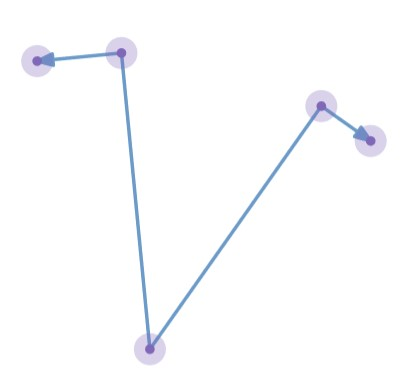
\includegraphics{angular_constraint.jpg}
\begin{gather}
C = \theta_a - \theta_b \\
\dot C = \omega_a - \omega_b \\
J = \begin{bmatrix}0 & 0 & 1 & 0 & 0 & -1\end{bmatrix} \\
JMJ^T = i_a + i_b
\end{gather}
\end{document}